\documentclass[cn,hazy,green,12pt,normal]{elegantnote}

\title{作业4解答}
\author{24Spring 回归分析}
\date{\today}

\usepackage{array}

\usepackage{amsmath, amssymb, bm, color, framed, graphicx, hyperref, mathrsfs, fontspec, geometry, extarrows, amsthm}

\DeclareMathOperator{\e}{\!\!\;\mathrm e}
\DeclareMathOperator{\Cov}{Cov}
\DeclareMathOperator{\Var}{Var}
\DeclareMathOperator{\var}{var}
\DeclareMathOperator{\tr}{tr}
\DeclareMathOperator{\diag}{diag}
\newcommand{\p}{\partial}
\renewcommand{\d}{\mathop{}\!\mathrm{d}}
\newcommand{\MR}{\mathbb R}
\newcommand{\MC}{\mathbb C}
\newcommand{\MF}{\mathbb F}
\newcommand{\MZ}{\mathbb Z}
\newcommand{\MN}{\mathbb N}
\newcommand{\MCF}{\mathscr F}
\renewcommand{\Re}{\operatorname{Re}}
\renewcommand{\Im}{\operatorname{Im}}
\renewcommand{\boldsymbol}{\bm}
\renewcommand{\i}{\mathrm i}

\DeclareMathOperator{\Arg}{Arg}
\DeclareMathOperator{\I}{I}
\usepackage{tkz-euclide}
\numberwithin{equation}{section}
\numberwithin{subsection}{section}

\lstset{
    language=R,
    basicstyle=\ttfamily,
    keywordstyle=\color{blue},
    commentstyle=\color{gray},
    frame=single,
    breaklines=true
}

\begin{document}
\maketitle

\begin{homework}   
\end{homework}
题干略,题目如下:
    \begin{figure}[!htbp]
        \centering
        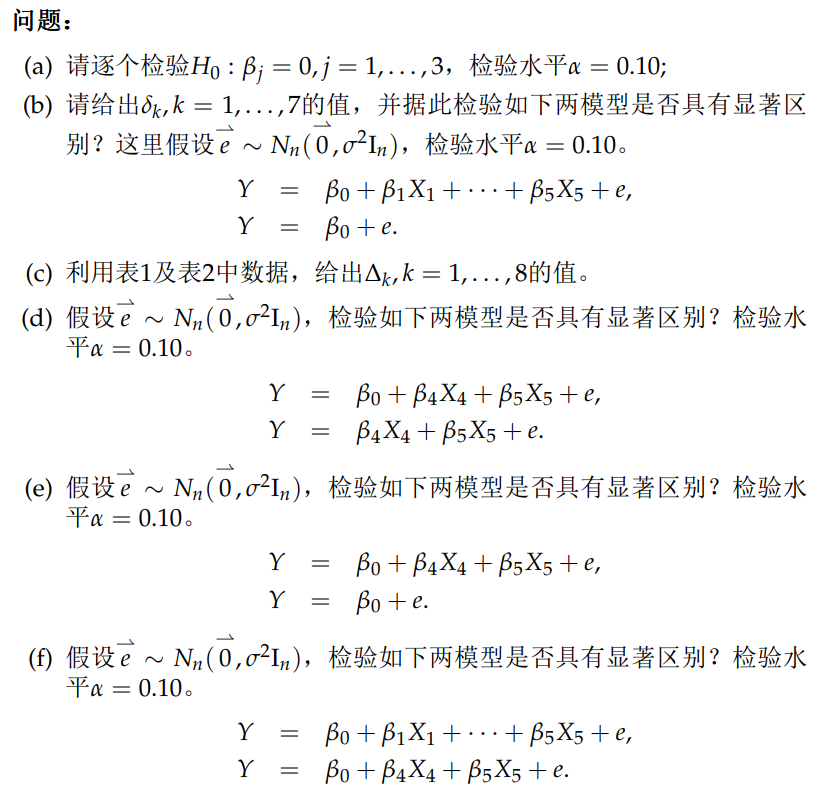
\includegraphics[width=30em]{image/hw4_plt1.png}
    \end{figure}

\begin{proof}[\solutionname]
    \textbf{题目修改:不用求}$\triangle_4$。
\end{proof}
(a) 可以选用t检验或者方差分析中的F检验。以t检验为例:
对\[H_0: \beta_1 = 0\]
有$\hat{\beta_1} \sim N(\beta_1, d_1^T\sigma^2(X_c^TX_c)^{-1}d_1)=N(\beta_1, c_{11})$
,由课上定理3.1.1得
\[t_1 = \dfrac{\hat{\beta_1}}{\hat{\sigma}\sqrt{c_{11}}}\overset{H_0}{\sim} t_{n-p}\]
代入$\hat{\sigma}= \sqrt{\hat{\sigma}^2} = \sqrt{RSS/(n-p)}=\sqrt{4816}=69.3974$(由题目表格得到MS=4816),

$\hat{\beta_1}=1.202,c_{11}=0.068\times10^{-2},n= 38,p=6$得到$t_1=0.66$。

由$|t_1|<t_{32}(0.05)=1.69$,故接受$H_0$。

类似求解$t_2=-0.26,\quad t_3 = 0.56$可知均接受$H_0$。

\noindent (b) 自由度:$\delta_1 = p-1=5, \quad \delta_5=n-p=32, \quad \delta_7=n-1=37$

SS:$\delta_6 = \delta_5\times MS=154112,\quad \delta_2=SYY-RSS=216571-154112=62459$

MS:$\delta_3 = \dfrac{\delta_2}{\delta_1}=12491.8$

F:$\delta_4 = \dfrac{\delta_3}{4816} = 2.5938$

这里是回归方程检验,直接用表中的F统计量$\delta_4$。由$\delta_4>2.036=F_{5,32}(0.1)$,故否定$H_0$,认为模型有显著差别。

\noindent (c) 自由度:$\triangle_1=2,\quad \triangle_5 = 3$

SS:$\triangle_2 = (y^TX_c)_{4,5}([X_c^TX_c]_{4,5})^{-1}(X_c^Ty)_{4,5}$,其中下标表示截取对应分量或者主子矩阵。

$X_c^T y=X_c^T(\hat{y}+\hat{e})=X_c^T\hat{y}=X_c^T(\bm 1 \bar{y} + X_c\hat{\beta}_c)=X_c^TX_c\hat{\beta}_c$\footnote{或者利用$\hat{\beta}_c = (X_c^T X_c)^{-1}X_c^Ty$,两边同左乘$X_c^T X_c$}两侧同时取第4,5分量,得到

\[(X_c^Ty)_{4,5}=(X_c^TX_c)_{[4:5,]}\hat{\beta}_c=
\begin{bmatrix}
    67.303& 1.416& 17.434& 8.661 & 2.092 \\
    64.485 & 35.222 & -5.446 & 2.092 & 160.700\\
\end{bmatrix}\begin{bmatrix}
    1.202\\
    -4.868\\
    6.109\\
    35.407\\
    10.978\\
\end{bmatrix}=\begin{bmatrix}
    510.139\\
    1711.017\\
\end{bmatrix}
\]
$\triangle_2 = [510.139,1711.017]\begin{bmatrix}
    8.661 & 2.092\\
    2.092 & 160.700\\
\end{bmatrix}^{-1}\begin{bmatrix}
    510.139\\
    1711.017\\
\end{bmatrix}=45785.26$

$\triangle_6 = SS_{reg}-SS_{reg}^{4,5}=\delta_2 - \triangle_2 = 16673.74$

MS(除以对应自由度):$\triangle_3 = 22892.63 ,\quad \triangle_7 = 5557.913$

F:$\triangle_4=\dfrac{\triangle_3}{\hat{\sigma}^2}=4.75 ,\quad \triangle_8=\dfrac{\triangle_7}{\hat{\sigma}^2}=1.15$

(d) 检验截距,利用公式$c_{00}=\frac{1}{n} + (m_4, m_5)([X_c^TX_c]_{4,5})^{-1}\begin{bmatrix}
    m_4\\
    m_5\\
\end{bmatrix}=  2.879462$

$\bar{y}=224$(将x均值代入最开始拟合方程。)

此模型下的$\beta_0$的OLS估计为
\[\tilde{\beta}_0=\Bar{y}-(m_4, m_5)\tilde{\beta}\footnote{这里$\tilde{\beta}$定义与注(1)相同}=\bar{y}-(m_4, m_5) ([X_c^TX_c]_{4,5})^{-1}(X_c^Ty)_{4,5}=-100
\]

$\tilde{\sigma}^2 = \dfrac{RSS^{4,5}}{n-3}= 4879.5971\quad t = \dfrac{\tilde{\beta}_0}{\tilde{\sigma}\sqrt{c_{00}}}=-0.8436312$

由$|t|=0.8436312<1.689572 = t_{35} (0.05)$,故认为该水平下无显著区别。

(e) 相当于检验回归方程显著性。
\[F = \dfrac{SS_{reg}^{4,5}/2}{\tilde{\sigma}^2}=4.69 > 2.460936=F_{2, 35}(0.10)\]
故该水平下有显著区别。

(f)$H_0: \beta_1 = \beta_2 = \beta_3 = 0$,即考虑经过$X_4,X_5$调整后的模型,关于$X_1,X_2,X_3$的回归。

\[F = \dfrac{(RSS_H-RSS)/3}{RSS/n-6}=\triangle_8=1.15 < 2.263=F_{3,32}(0.10)\]
故该水平下无显著区别。


\begin{note}
    (1)C问中计算$\triangle_2$的值($SS_{reg}^{4,5}$)时,有$SS_{reg}^{4,5}=||X_{c(4,5)}\tilde{\beta}||^2$,其中$\tilde{\beta}$为模型
    \[Y = \beta_0 + \beta_4X_4 + \beta_5X_5+e\]
    中$(\beta_4,\beta_5)$的LS估计。这与全模型中$\hat{\beta_c}$的第4、5个分量是不一样的。因此不能简单截取全模型中LS估计$\hat{\beta_c}$的若干分量计算。

    \noindent(2)这题后面几问都涉及到注(1)中的模型比较,计算比较繁琐,不要与原模型下的一些估计搞混,
\end{note}

\newpage

\begin{homework}
\end{homework}

    \begin{figure}[!htbp]
        \centering
        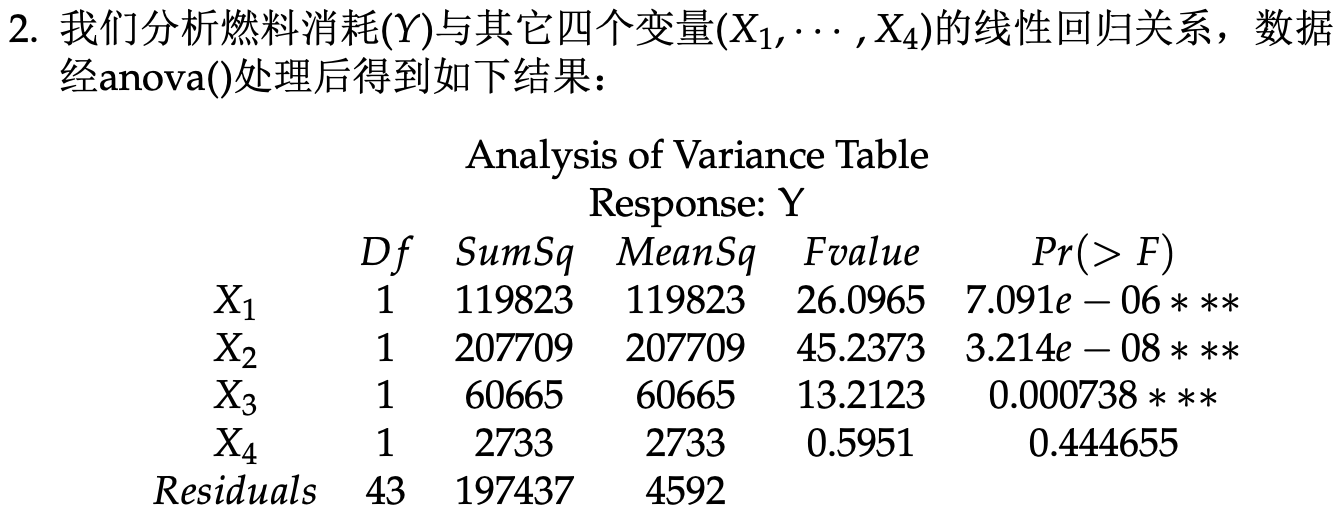
\includegraphics[width=30em]{image/hw4_plt21.png}
    \end{figure}

    \begin{figure}[!htbp]
        \centering
        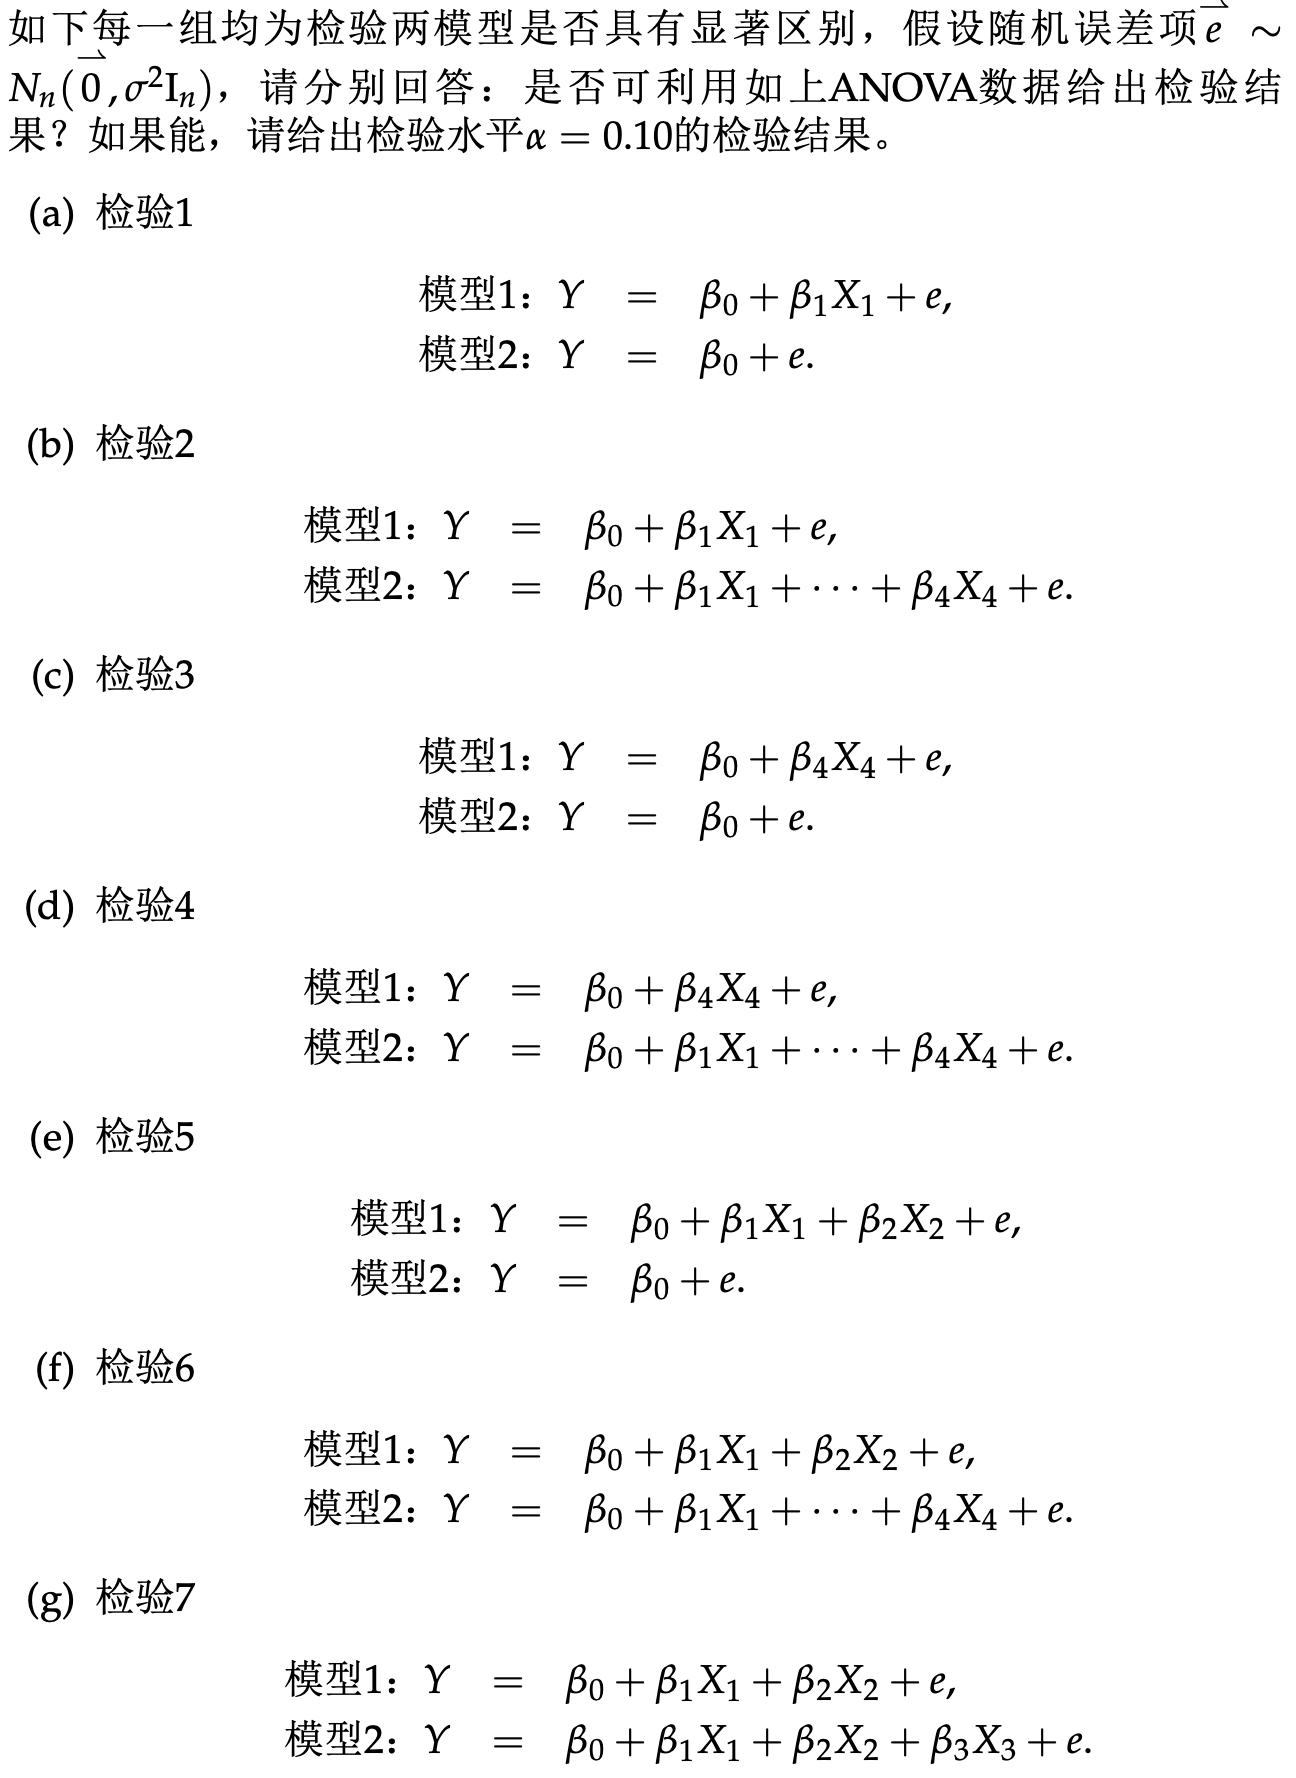
\includegraphics[width=30em]{image/hw4_plt22.png}
    \end{figure}

\begin{proof}[\solutionname]
\end{proof}

本题要求我们判断是否可利用序贯方差分析表中的数据检验两模型是否有显著区别,并给出检验结果。利用课件第三章第2节公式(3)给出检验统计量
$$
F_H = \frac{(RSS_H - RSS)/m}{RSS/(n-p)},
$$
其中$n=48$,$p,m$由具体的检验问题给出,$RSS$是包含较多变量的模型的残差平方和,$RSS_H$是包含较少变量的模型的残差平方和。判断能否给出两模型是否有显著区别的检验,只需要判断能否从序贯方差分析表中得到相应的$RSS,RSS_H$。沿用课件的记号,当$I$为变量的指标集时,$SS_{reg}^I$为包含相应变量的模型的回归平方和。根据序贯方差分析表中的数据
\begin{align*}
    119823 &= SS_{reg}^1 \\
    207709 &= SS_{reg}^{1,2} - SS_{reg}^{1} \\
    60665 &= SS_{reg}^{1,2,3} - SS_{reg}^{1,2} \\
    2733 &= SS_{reg}^{1,2,3,4} - SS_{reg}^{1,2,3} \\
    197437 &= SYY - SS_{reg}^{1,2,3,4}
\end{align*}
依次累加可分别得到$SS_{reg}^{1},SS_{reg}^{1,2},SS_{reg}^{1,2,3},SS_{reg}^{1,2,3,4},SYY$,再由$SYY = SS_{reg} + RSS$可得相应的$RSS$。

(a)$RSS = SYY - SS_{reg}^1 = 207709 + 60665 + 2733 + 197437$,$RSS_H - RSS = SS_{reg}^1 = 119823$,则
$$
F_H = \frac{119823 / 1}{(207709 + 60665 + 2733 + 197437) / (48-2)} = 11.76 > 2.82 = F_{1,46}(0.10)
$$
认为两模型有显著区别。

(b)$RSS = SYY - SS_{reg}^{1,2,3,4} = 197437$,$RSS_H - RSS = SS_{reg}^{1,2,3,4} - SS_{reg}^1 = 207709 + 60665 + 2733$,则
$$
F_H = \frac{(207709 + 60665 + 2733) / 3}{197437 / (48-5)} = 19.68 > 2.22 = F_{3,43}(0.10)
$$
认为两模型有显著区别。

(c)(d)因为无法从上述ANOVA数据中得到$SS_{reg}^4$,则无法得到模型$Y = \beta_0 + \beta_4 X_4 + e$的残差平方和,这两个问题均无法检验。

(e)$RSS = SYY - SS_{reg}^{1,2} = 60665 + 2733 + 197437$,$RSS_H - RSS = SS_{reg}^{1,2} = 119823 + 207709$,则
$$
F_H = \frac{(119823 + 207709) / 2}{(60665 + 2733 + 197437) / (48-3)} = 28.25 > 2.42 = F_{2,45}(0.10)
$$
认为两模型有显著区别。

(f)$RSS = SYY - SS_{reg}^{1,2,3,4} = 197437$,$RSS_H - RSS = SS_{reg}^{1,2,3,4} - SS_{reg}^{1,2} = 60665 + 2733$,则
$$
F_H = \frac{(60665 + 2733) / 2}{197437 / (48-5)} = 6.90 > 2.43 = F_{2,43}(0.10)
$$
认为两模型有显著区别。

(g)$RSS = SYY - SS_{reg}^{1,2,3} = 2733 + 197437$,$RSS_H - RSS = SS_{reg}^{1,2,3} - SS_{reg}^{1,2} = 60665$,则
$$
F_H = \frac{60665 / 1}{(2733 + 197437) / (48-4)} = 13.33 > 2.82 = F_{1,44}(0.10)
$$
认为两模型有显著区别。


\newpage

\begin{homework}
\end{homework}

    \begin{figure}[!htbp]
        \centering
        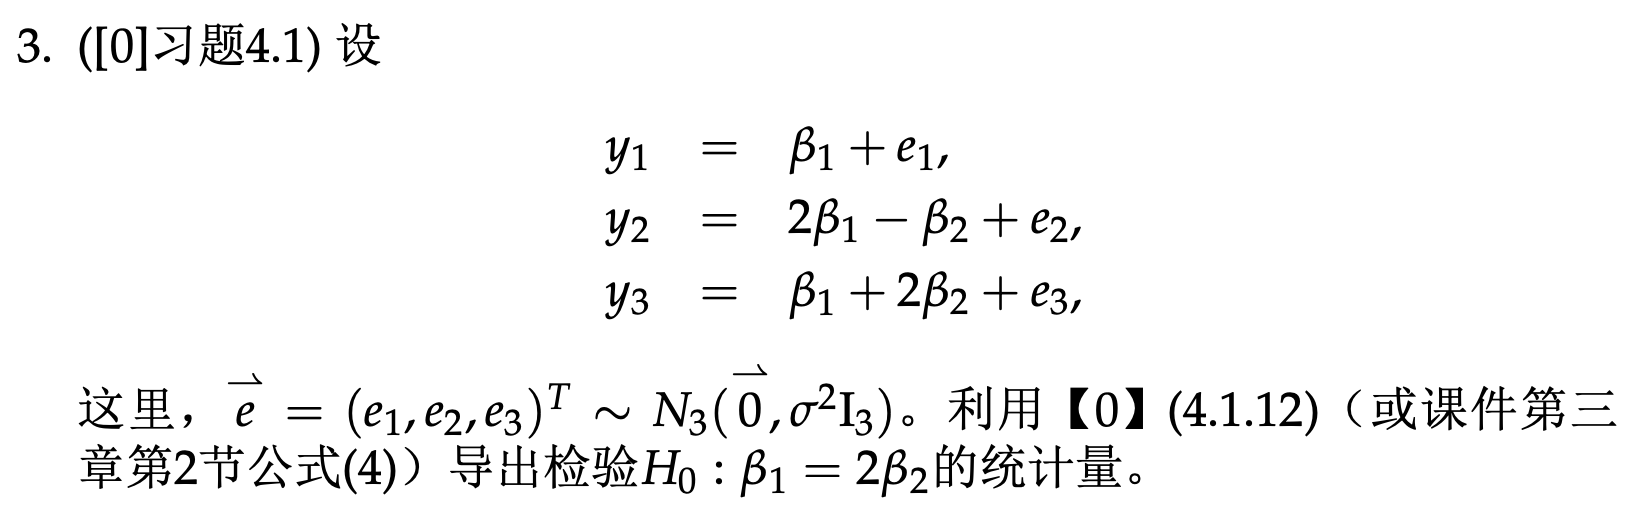
\includegraphics[width=30em]{image/hw4_plt3.png}
    \end{figure}

\begin{proof}[\solutionname]
\end{proof}

利用课件第三章第2节公式(4),
$$
F_H = \frac{(A \hat{\beta} - b)^T (A(X^T X)^{-1}A^T)^{-1} (A \hat{\beta} - b) / m}{\hat{\sigma}^2}
$$
其中
\begin{gather*}
A = 
\begin{pmatrix}
1 & -2    
\end{pmatrix}
\quad b = 0 \quad m = rank(A) = 1 \\
X = 
\begin{pmatrix}
    1 & 0 \\
    2 & -1  \\
    1 & 2
\end{pmatrix}
\quad y = 
\begin{pmatrix}
    y_1 \\
    y_2 \\
    y_3
\end{pmatrix} \\
\hat{\beta} = (X^T X)^{-1} X^T y \\
\hat{\sigma}^2 = \frac{RSS}{n-p} = y^T(I-X(X^T X)^{-1}X^T)y = y^T y - y^T X \hat{\beta}
\end{gather*}
代入后可导出检验统计量
$$
F_H = \frac{30}{29} \cdot \frac{(\frac{1}{6}y_1 + \frac{11}{15}y_2 - \frac{19}{30}y_3)^2}{\frac{5}{6}y_1^2 + \frac{2}{15}y_2^2 + \frac{1}{30}y_3^2 - \frac{2}{3}y_1y_2 - \frac{1}{3}y_1y_3 + \frac{2}{15}y_2y_3}.
$$

\begin{note}
    (1)在上述解答中,相关计算步骤被省略了,作业与考试里还是必须要有完整的计算过程,否则可能会被扣分。
    
    \noindent (2)此题模型中没有截距项,不要计算成$X_c$了。
\end{note}

\newpage

\begin{homework}
\end{homework}

    \begin{figure}[!htbp]
        \centering
        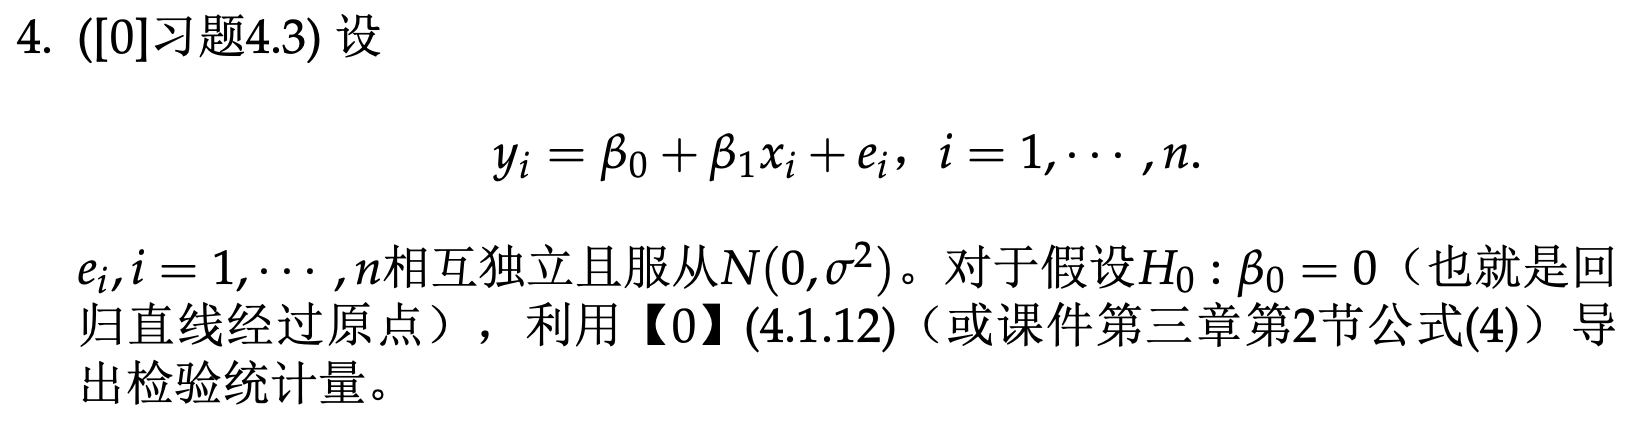
\includegraphics[width=30em]{image/hw4_plt4.png}
    \end{figure}

\begin{proof}[\solutionname]
\end{proof}

利用课件第三章第2节公式(3),
$$
F_H = \frac{(RSS_H - RSS)/m}{RSS/(n-p)},
$$
其中$m=1$,$p=2$,$RSS$为无约束模型(此处是带截距项模型)的残差平方和,
$$
RSS = SYY - \frac{(SXY)^2}{SXX},
$$
$RSS_H$为有约束模型(此处是无截距模型)的残差平方和,
$$
RSS_H = SYY + n \bar{y}^2 - \frac{SXY + n \bar{x} \bar{y}}{SXX + n \bar{x}^2}.
$$
将$RSS$与$RSS_H$的式子代入$F_H$的表达式即可导出检验统计量。

\begin{note}
    (1)关于一元线性回归模型在有截距、无截距情形下残差平方和的公式,可参考作业2解答。

    \noindent (2)或者用t检验,$\hat{\beta}_0=\bar{y}-\dfrac{SXY}{SXX}\bar{x}, c_{00} = \frac{1}{n} + \dfrac{\bar{x}^2}{SXX}, \hat{\sigma}^2 = RSS/n-2, t = \dfrac{\hat{\beta}_0}{\hat{\sigma}\sqrt{c_{00}}}\overset{H_0}{\sim}t_{n-2}$
\end{note}

\newpage

\begin{homework}
\end{homework}

    \begin{figure}[!htbp]
        \centering
        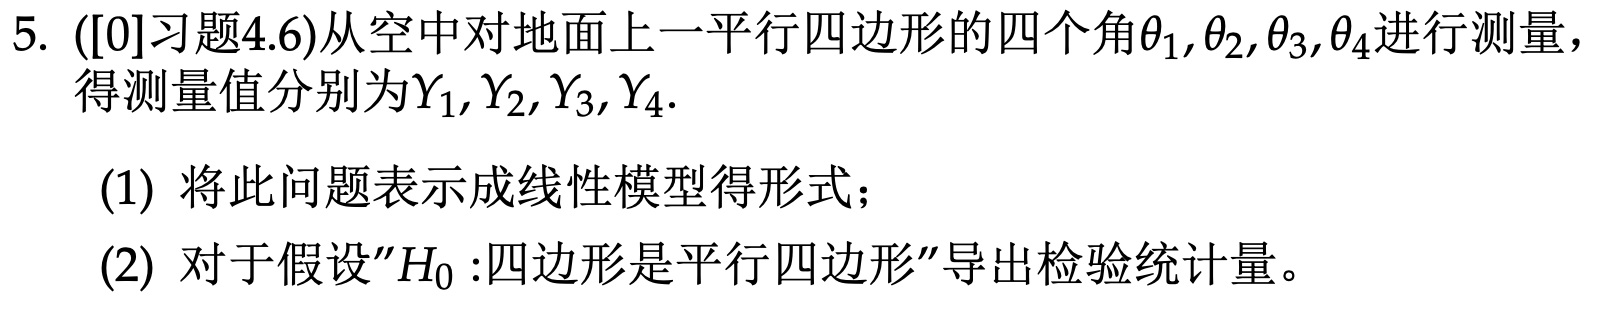
\includegraphics[width=30em]{image/hw4_plt5.png}
    \end{figure}

\begin{proof}[\solutionname]
\end{proof}

(1)注意到四边形的四个角之和为360度,则可只考虑$\theta_1,\theta_2,\theta_3$,
\begin{align*}
    Y_1 &= \theta_1 + e_1 \\
    Y_2 &= \theta_2 + e_2 \\
    Y_3 &= \theta_3 + e_3 \\
    Y_4 &= 360 - \theta_1 - \theta_2 - \theta_3 + e_4
\end{align*}
记$(y_1,y_2,y_3,y_4) = (Y_1,Y_2,Y_3,Y_4-360)$,则问题可表示成线性模型
$$
y = X \theta + e
$$
其中
$$
y = \begin{pmatrix}
    y_1 \\
    y_2 \\
    y_3 \\
    y_4 
\end{pmatrix}, \
X = \begin{pmatrix}
    1 & 0 & 0 \\
    0 & 1 & 0 \\
    0 & 0 & 1 \\
    -1 & -1 & -1 
\end{pmatrix}, \
\theta = \begin{pmatrix}
    \theta_1 \\
    \theta_2 \\
    \theta_3 
\end{pmatrix}, \
e = \begin{pmatrix}
    e_1 \\
    e_2 \\
    e_3 \\
    e_4 
\end{pmatrix}, \
e \sim N(0,\sigma^2 I).
$$

(2)导出检验统计量利用课件第三章第2节公式(3),
$$
F_H = \frac{(RSS_H - RSS)/m}{RSS/(n-p)}.
$$
先考虑分母,$n=4,\ p=3$,$RSS$是上述线性模型的残差平方和
\begin{align*}
    RSS =& y^T (I - X(X^T X)^{-1}X^T) y \\
    =& \frac{1}{4} Y_1^2 + \frac{1}{4} Y_2^2 + \frac{1}{4} Y_3^2 + \frac{1}{2} Y_1 Y_2 + \frac{1}{2} Y_1 Y_3 + \frac{1}{2} Y_2 Y_3 \\
    &+ \frac{1}{4} (Y_4-360)^2 + \frac{1}{2} Y_1 (Y_4-360) + \frac{1}{2} Y_2 (Y_4-360) + \frac{1}{2} Y_3 (Y_4-360).
\end{align*}
接下来考虑分子,“四边形是平行四边形”的假设等价于在
$$
\theta_1 + \theta_2 = 180, \ \theta_1 - \theta_3 = 0,
$$
故$m = 2$。在原假设成立的条件下,
\begin{align*}
    Y_1 &= \theta_1 + e_1 \\
    Y_2 &= 180 - \theta_1 + e_2 \\
    Y_3 &= \theta_1 + e_3 \\
    Y_4 &= 180 - \theta_1 + e_4
\end{align*}
记$(y_1,y_2,y_3,y_4) = (Y_1,Y_2-180,Y_3,Y_4-180)$,此时的线性模型为
$$
y = X \theta_1 + e
$$
其中
$$
y = \begin{pmatrix}
    y_1 \\
    y_2 \\
    y_3 \\
    y_4 
\end{pmatrix}, \
X = \begin{pmatrix}
    1 \\
    -1 \\
    1 \\
    -1 
\end{pmatrix}, \
e = \begin{pmatrix}
    e_1 \\
    e_2 \\
    e_3 \\
    e_4 
\end{pmatrix}, \
e \sim N(0,\sigma^2 I).
$$
$RSS_H$是该线性模型的残差平方和,则
\begin{align*}
    RSS_H =& y^T (I - X(X^T X)^{-1}X^T) y \\
    =& \frac{3}{4} Y_1^2 + \frac{3}{4} (Y_2-180)^2 + \frac{3}{4} Y_3^2 + \frac{3}{4} (Y_4-180)^2 + \frac{1}{2} Y_1 (Y_2-180) -\frac{1}{2} Y_1 Y_3 \\
    &+ \frac{1}{2} (Y_2-180) Y_3 + \frac{1}{2} Y_1 (Y_4-180) - \frac{1}{2} (Y_2-180)(Y_4-180) + \frac{1}{2} Y_3 (Y_4-180).
\end{align*}
将$RSS,RSS_H$的计算结果代入$F_H$的表达式可得
$$
F_H = \frac{(Y_1-Y_3)^2+(Y_2-Y_4)^2}{(Y_1+Y_2+Y_3+Y_4-360)^2}.
$$

\newpage

\begin{homework}
\end{homework}

题干略,问题如下:

    \begin{figure}[!htbp]
        \centering
        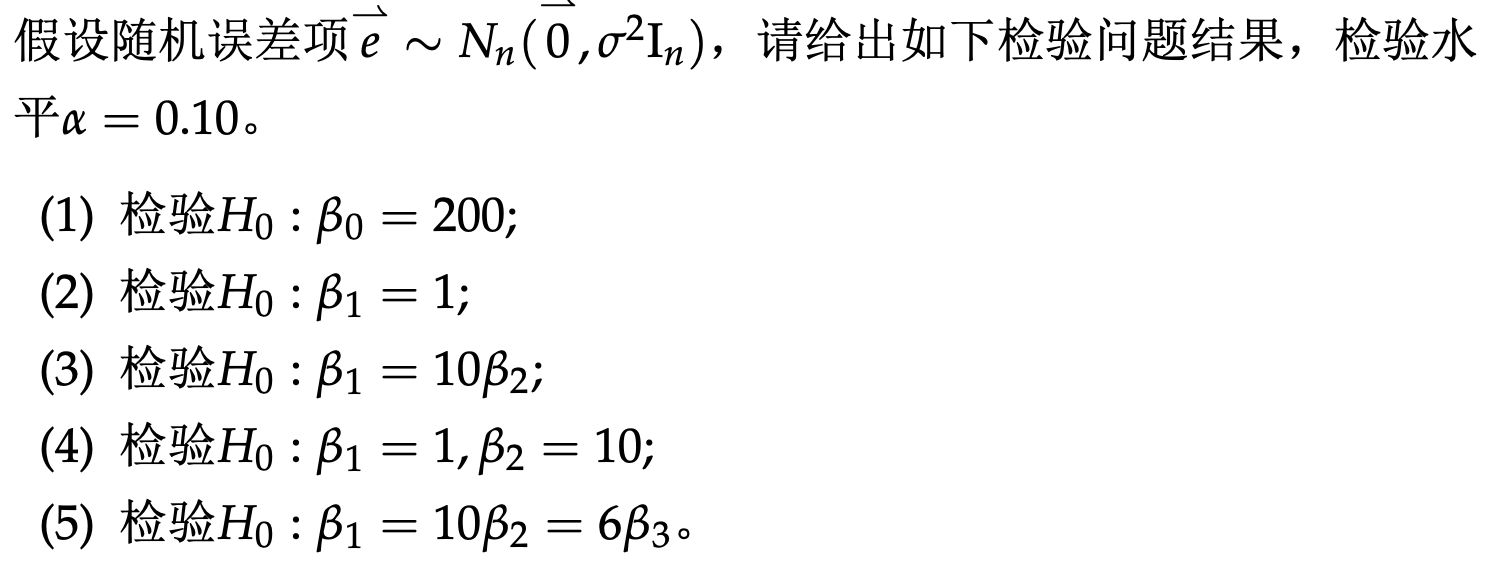
\includegraphics[width=30em]{image/hw4_plt6.png}
    \end{figure}

\begin{proof}[\solutionname]
\end{proof}

(1)利用课件第三章第2节公式(4),
$$
F_H = \frac{(A \hat{\beta} - b)^T (A(X^T X)^{-1}A^T)^{-1} (A \hat{\beta} - b) / m}{\hat{\sigma}^2}
$$
其中$\hat{\beta} = 
\begin{pmatrix}
    175.271 & 1.348 & 10.095 & 6.315
\end{pmatrix}^T, \ \hat{\sigma}^2 = 72.53$题干已给出,此处$A = 
\begin{pmatrix}
    1 & 0 & 0 & 0
\end{pmatrix}, \ b = 200, \ m = rank(A) = 1$,且$A(X^T X)^{-1}A^T = [(X^T X)^{-1}]_{1,1} = \frac{1}{n} + m^T (Xc^TXc)^{-1} m$,代入题干中的数值可得,
$$
F_H = 33.28 > 2.86 = F_{1,34}(0.10)
$$
故拒绝$H_0$。

接下来的几个检验不涉及截距项,则可利用中心化模型下的检验统计量
$$
F_H = \frac{(A \hat{\beta}_c - b)^T (A(X_c^T X_c)^{-1}A^T)^{-1} (A \hat{\beta}_c - b) / m}{\hat{\sigma}^2}
$$
其中$\hat{\beta}_c, (X_c^T X_c)^{-1}, \hat{\sigma}^2$在题干中已给出,只需将每个检验问题对应的$A,b,m$代入公式计算,再与临界值做比较即可。

(2)$F_H = 2.50 < 2.86 = F_{1,34}(0.10)$,故接受$H_0$。

(3)$F_H = 29.99 > 2.86 = F_{1,34}(0.10)$,故拒绝$H_0$。

(4)$F_H = 1.29 < 2.47 = F_{2,34}(0.10)$,故接受$H_0$。

(5)$F_H = 31.63 > 2.47 = F_{2,34}(0.10)$,故拒绝$H_0$。

\begin{note}
    (1)在上述解答中,相关计算步骤被省略了,这是因为它的流程比较固定、只需套公式。作业与考试里还是必须要有完整的计算过程,否则可能会被扣分。

    \noindent (2)第三问如果改为$H_0: \beta_1=\dfrac{1}{10}\beta_2$,则计算得$F_H=1.663$接受原假设。
\end{note}


\end{document}

